%\documentclass[11pt]{beamer}
\documentclass[10pt, hyperref={unicode}]{beamer}
\usepackage[czech]{babel}
\usepackage[utf8]{inputenc}
\usepackage{times}
\usepackage{graphicx}

\usetheme{Madrid}
\usecolortheme{whale}

\title{Konečné automaty}
\author{Nikolas Masica}
\institute{VUT FIT}
\date{2018}

\begin{document}
\maketitle
\begin{frame}{Přehled}
	\tableofcontents
\end{frame}

\section{Definice}

\begin{frame}{Definice}
\begin{itemize}
    \item Konečný automat je teoretický výpočetní model používaný v informatice pro studium formálních jazyků.
    \item Popisuje velice jednoduchý počítač, který může být v jednom z několika stavů, mezi kterými přechází na základě symbolů, které čte ze vstupu.
    \item Konečný automat je velice jednoduchý výpočetní model, dokáže rozpoznávat pouze regulární jazyky. Konečné automaty se používají při vyhodnocování regulárních výrazů
\end{itemize}
\end{frame}

\section{Formální definice}
\begin{frame}{Formální definice}
Formálně je konečný automat definován jako uspořádaná pětice $(S,\Sigma,\sigma ,s,A)$, kde:
\begin{itemize}
    \item $S$ je konečná neprázdná množina stavů.
    \item $\Sigma$ je konečná neprázdná množina vstupních symbolů, nazývaná abeceda
    \item $\sigma$ je tzv. přechodová funkce, popisující pravidla přechodů mezi stavy. Může mít buď podobu $S \times \Sigma \rightarrow S$, nebo $S \times \{\Sigma \cup \varepsilon \} \rightarrow P(S)$
    \item $s$ je počáteční stav, $s \in S$.
    \item $A$ je množina přijímajících stavů, $A \subseteq S$.
\end{itemize}
\end{frame}
\section{Popis činnosti automatu}
\begin{frame}{Popis činnosti automatu}
\begin{itemize}
    \item Na počátku se automat nachází v definovaném počátečním stavu.
    \item V každém kroku přečte jeden symbol ze vstupu a přejde do stavu, který je dán hodnotou, která v přechodové tabulce odpovídá aktuálnímu stavu a přečtenému symbolu.
    \item Pokračuje čtením dalšího symbolu ze vstupu, dalším přechodem podle přechodové tabulky atd.
    \item Podle toho, zda automat skončí po přečtení vstupu ve stavu, který patří do množiny přijímajících stavů, platí, že automat buď daný vstup přijal, nebo nepřijal.
    \item Množina všech řetězců, které daný automat přijme, tvoří regulární jazyk.
\end{itemize}
\end{frame}

\section{Deterministický konečný automat}
\begin{frame}{Deterministický konečný automat}
\begin{itemize}
    \item Deterministický konečný automat je charakteristický tím, že se vždy nachází právě v jednom ze svých vnitřních stavů.
    \item Deterministický konečný automat je uspořádaná pětice $(Q,Q_0,F,X,\delta)$ , kde:
        \begin{itemize}
            \item $Q:|Q| < \infty$ je konečná množina vnitřních stavů.
            \item $Q_0:Q_0 \in Q$ je počáteční stav.
            \item $F:F \subseteq Q$ je množina koncových stavů.
            \item $X:|X| < \infty$ je konečná vstupní abeceda.
            \item $\delta:Q \times X \rightarrow Q$ je přechodová funkce.
        \end{itemize}
\end{itemize}
\end{frame}

\section{Nedeterministický konečný automat}
\begin{frame}{Nedeterministický konečný automat}
\begin{itemize}
    \item Nedeterministický konečný automat je charakteristický tím, že se může v jednom okamžiku nacházet v celé množině svých vnitřních stavů. Nedeterministické konečné automaty lze převést na deterministické, avšak počet stavů se zvýší.
    \item Nedeterministický konečný automat je uspořádaná pětice $(Q,Q_0,F,X,\delta)$ , kde:
        \begin{itemize}
            \item $Q:|Q| < \infty$ je konečná množina vnitřních stavů.
            \item $Q_0:Q_0 \subseteq Q \wedge Q_0 \neq \emptyset$ je počáteční stav.
            \item $F:F \subseteq Q$ je množina koncových stavů.
            \item $X:|X| < \infty$ je konečná vstupní abeceda.
            \item $\delta:Q \times X \rightarrow P(Q)$ je přechodová funkce.
        \end{itemize}
\end{itemize}
\end{frame}

\section{Znázornění konečného automatu}
\begin{frame}{Znázornění konečného automatu}
\begin{itemize}
    \item Místo relativně nepřehledného popisu konečného automatu přímo tabulkou se obvykle používá grafické znázornění, na kterém kolečka znázorňují jednotlivé stavy a šipky mezi těmito kolečky popisují jednotlivé přechody.
\end{itemize}
\end{frame}

\begin{frame}{Znázornění konečného automatu}

	\begin{figure}[h]
		\centering
		\scalebox{0.4}{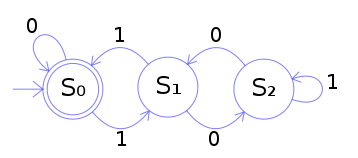
\includegraphics{automat.png}}
	\end{figure}
\begin{itemize}
    \item Dvojité kolečko označuje přijímající stavy, počáteční stav je označen šipkou směřující z volného prostoru k počátečnímu stavu, někdy s připsaným textem, např. START.
\end{itemize}
\end{frame}
\begin{frame}{Použité zdroje}
	\begin{thebibliography}{10}
		\bibitem[Wikipedia]{wiki} Wikipedia
		\newblock \texttt{https://cs.wikipedia.org/wiki/Konečný-automat}
		
		\bibitem[Voho]{voho} Voho
		\newblock \texttt{http://voho.eu/wiki/konecny-automat/}
		
		\bibitem[Matematika.cz]{Matematika.cz} Matematika.cz
		\newblock \texttt{https://matematika.cz/konecny-automat}
		
	\end{thebibliography}
\end{frame}
\end{document}
